\chapter{Serverless-Technologie}
\label{chap:serverless}

In diesem Kapitel geht es um eine Beschreibung und Abgrenzung der Grundbegriffe Serverless-Technologie und Reaktives System, sowie eine Einordnung der Zusammenhänge dieser Domänen.

\section{Was ist Serverless-Technologie?}
Serverless ist laut Red Hat ein „cloudnatives Entwicklungsmodell, bei dem Entwickler Anwendungen erstellen und ausführen können, ohne Server verwalten zu müssen” \cite{RedhatServerless}. Hier wird deutlich, dass der Begriff Serverless die Perspektive von Konsumenten und nicht von Anbietern dieser Technologieform beschreibt, da im physikalischen Sinne dennoch Server eingesetzt und verwaltet werden. Durch die Abstraktion generischer Problemfelder wird jedoch der Zugang dazu, insbesondere im Kontext der in der Vergangenheit etablierten On-Premise Lösungen, auf eine zielgerichtete Weise geschmälert und seitens des Betreibers mehr Verantwortung übernommen. Dies ist aus Entwicklersicht wertschöpfend, da man sich durch die Verwendung von Serverless-Technologie auf die Entwicklung von Geschäftslogik fokussieren kann, während Themen wie Betriebssysteme, Backups, Laufzeitumgebungen und Skalierung ausgelagert wird. Der Begriff ist nicht scharf genug definiert, um zu beinhalten, ab welcher Abstraktionsschicht eine Dienstleistung als Serverless bezeichnet werden darf, so definiert Redhat beispielsweise auch Container-as-a-Service als Serverless \cite{RedhatServerless}, während umgangssprachlich häufig eher höhere Abstraktionsstufen wie z.B. Function-as-a-Service damit assoziiert werden.

\section{Frontend im Kontext von Serverless-Technologie}
Der Begriff von Serverless-Technologie bezieht sich nicht direkt auf die Implementierung des Frontends, welches auf dem Gerät des Entanwenders ausgeführt wird (z.B. als App oder als Web-Applikation in einem Browser). Dennoch kann sich der Stil der Frontendentwicklung dadurch tangiert werden, dass Geschäftslogik, welche keine sicherheitskritischen Informationen beinhaltet, in einem solchen Kontext eher direkt im Frontend abgebildet wird. Dies erfordert unter Umständen komplexere Strukturen und den bewussten Einsatz von Architekturen und Entwurfsmustern innerhalb des Frontends.

\section{Function-as-a-Service (FaaS)}
Mit dem Begriff der Function-as-a-Service ist gemeint, dass der Betrieb einer Laufzeitumgebung für die Ausführung einer Programmfunktion auf generische Weise von einem Cloudanbieter zur Verfügung gestellt wird. Ein Entwickler kann diese Dienstleistung nutzen, indem er seinen Code zum Cloudanbieter hochlädt, und dafür eine eindeutige Adresse erhält, anhand welcher diese Funktion zu finden und auszuführen ist. Die Funktion ist dabei frei von Seiteneffekten, welche das Dateisystem, das Betriebssystem oder die Laufzeitumgebung betreffen, kann aber beispielsweise Berechnungen, Datenbankanfragen oder Anfragen an andere Funktionen durchführen. Ergibt sich durch gehäufte Anfragelast eine Überforderung des Servers, auf welchem die Funktion ausgeführt wird, so sorgt der Cloudanbieter automatisch für eine elastische Skalierung. Das Besondere dabei ist, dass dabei durchaus auch auf 0 skaliert werden kann, was bedeutet, dass der Container oder die Laufzeitumgebung, in welcher die Funktion ausgeführt wird, gestoppt wird. In dem Fall wird dann bei Wiederausführung erst die benötigte Infrastruktur gestartet, und daraufhin die Funktion ausgeführt. Dies wird als cold start bezeichnet. Kosten werden in Abhängigkeit von der Anzahl der Aufrufe geltend gemacht, wobei häufig üppige kostenfreie Kontingente zur Verfügung stehen. Dadurch ermöglicht FaaS das kostengünstige Ausprobieren von Features, ohne initiale Investitionen in das Aufsetzen von Servern zu erfordern.

\section{Reaktive Systeme}
\label{sec:res}
\subsection{Antwortbereitschaft}
Reaktive Systeme verfolgen das Ziel, zu jeder Zeit und gleichzeitig für beliebig viele Nutzer antwortbereit zu sein. Dafür werden drei weitere Qualitäten vorgeschrieben: Widerstandsfähigkeit, Elastizität sowie Nachrichtenorientiertheit, um die Antwortbereitschaft herzustellen \cite[vgl.][]{ReactiveManifesto}. Diese Begriffe sowie deren Zusammenhänge sollen im Folgenden erklärt werden, um einen Vergleich zwischen den Prinzipien dieser beiden Paradigmen zu ermöglichen. 

\subsection{Widerstandsfähigkeit}
Mit Widerstandsfähigkeit ist gemeint, dass das System „selbst bei Ausfällen von Hard- oder Software antwortbereit” \cite{ReactiveManifesto} bleibt. Erreicht wird dies durch Replikation, Delegation und Isolation. Die Replikation der Funktionalität, wie beispielsweise durch mehrere Instanzen einer Komponente, kann Fehler einzelner Komponenten auffangen, indem die Anfragelast auf die funktionierenden Komponenten umgeleitet wird. Die Delegation von Verantwortung greift beispielsweise dann, wenn ein Fehlerfall auftritt, dessen Handhabe nicht von der Komponente selbst erreicht werden kann. In dem Fall kann sie die Abarbeitung an andere Komponenten delegieren und so selbst wieder in einen funktionalen Zustand zurückkehren. Auch die Isolation zwischen den Komponenten ist ein wichtiger Aspekt für die Widerstandsfähigkeit eines Systems, da sie dafür sorgt, dass an einer Stelle auftretende Fehler sich nicht auf andere Komponenten auswirken kann. Durch hohe Isolation bleibt der Schaden, den ein System durch einen Hardware- oder Softwarefehler nehmen kann, auf einen definierten Bereich eingeschränkt.

\subsection{Elastizität}
Ein elastisches System ist eines, welches in Abhängigkeit von der momentanen Anfragelast den Umfang der genutzten Ressourcen automatisch dynamisch festlegt. Sich ändernde Anfragelasten sind etwas sehr übliches in der Softwarebranche, Beispiele sind Abhängigkeiten von der Tages- oder Jahreszeit, bestimmten Veranstaltungen oder Hypes. Ein Beispiel ist der angekündigte Release eines Spiels, bei dem es die Möglichkeit zur Vorbestellung gab. Ab dem Zeitpunkt der Veröffentlichung wird dann schlagartig von sehr vielen Spielern mit hohen Erwartungen das Spiel heruntergeladen, und es ist keine Seltenheit, dass die Server des Spieleherstellers in dem Moment Symptome der Überlastung zeigen\footnote{z.B. hier: \url{https://www.pcgamer.com/halo-infinite-steam-servers-slow/} und hier: \url{https://arstechnica.com/gaming/2021/11/rockstar-servers-down-for-nearly-a-day-amid-remastered-gta-trilogy-launch/}.}. Das bedeutet konkret, dass bei einer sehr hohen Anfragelast zusätzliche Ressourcen, etwa in Form von Servern oder Kubernetes Nodes, zusätzlich gestartet werden, und die Anfragelast entsprechend aufgeteilt wird. Fällt die Anfragelast, so können diese zusätzlichen Instanzen automatisch auch wieder aufgelöst werden, um die dafür anfallenden Kosten zu sparen. Damit ein System überhaupt elastisch sein kann, muss es jedoch erst einmal skalierbar sein, wofür seinerseits Vorbedingungen gelten. Eine dieser Vorbedingungen ist die Nachrichtenorientiertheit.

\subsection{Nachrichtenorientiertheit}
In der Welt der verteilten Systeme muss ein Weg gefunden werden, die einzelnen Komponenten zuverlässig und eindeutig miteinander kommunizieren zu lassen. Für reaktive Systeme bedeutet das, dass die Nachrichten zwischen den einzelnen Komponenten asynchron und entkoppelt sind. Eine konkrete Umsetzung einer solchen Architektur lässt sich beispielsweise mit Apache Kafka oder dem Closed Source Equivalent Simple Notification Service der AWS erreichen. Es werden Topics definiert, auf welche Nachrichten gesendet werden können. Dabei ist dem Sender der Nachricht nicht wichtig, welche Komponenten die versendete Nachricht entgegennehmen. Auf den Topics werden die Nachrichten persistiert, während Komponenten auf diese reagieren können. Der wichtige Aspekt dabei ist die Entkopplung zwischen dem Sender der Nachricht und dem Empfänger. Durch die Überwachung der Nachrichten als Queue kann sowohl das Auftreten von Fehlern beobachtet werden (eine Komponente arbeitet keine Nachrichten mehr ab), als auch geschlussfolgert werden, ob mehr oder weniger Ressourcen als zum aktuellen Zeitpunkt zur Verfügung stehen benötigt werden. Somit ermöglicht die Nachrichtenorientiertheit sowohl die Widerstandsfähigkeit als auch die Elastizität, während diese beiden Eigenschaften antwortbereite und somit reaktive Systeme ermöglichen (vgl. Abbildung \ref{fig:reac}).
\begin{figure}[H]
    \centering
    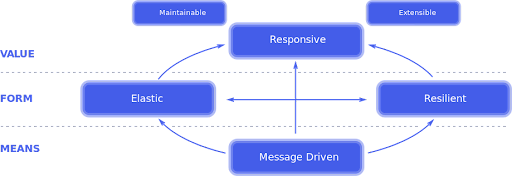
\includegraphics[width = .9\textwidth]{images/resy.png}
    \caption{ Die Darstellung der Abhängigkeiten der Qualitäten eines reaktiven Systems, \cite{ReactiveManifesto}}
    \label{fig:reac}
\end{figure}

\section{Reaktive Systeme und Serverless-Systeme}
\subsection{Gemeinsames Ziel: Antwortbereitschaft}
Die Zielstellung von reaktiven Systemen und von Serverless-Prinzipien haben einige Gemeinsamkeiten, unterscheiden sich aber vor allem in der Perspektive auf diese wünschenswerten Eigenschaften. Um diese Gemeinsamkeiten und Unterschiede herauszuarbeiten, soll ein Blick auf die generelle Wertschöpfungskette in der Erstellung von Software geworfen werden. Aus wirtschaftlicher Sicht verfolgen die meisten Softwaresysteme das Ziel, einen Mehrwert durch Problemllösung des Nutzers zu schaffen. Dies kann ein System nur dann erreichen, wenn es auch entsprechend zuverlässig, schnell und korrekt antwortet, sobald ein Nutzer eine Anfrage macht. Dieses Ziel ist entsprechend unabhängig von den beiden Paradigmen, kann aber auch als primäres Ziel von beiden verstanden werden. Der Fokus von reaktiven Systemen liegt dabei allerdings eher auf der Struktur von Serveranwendungen, während die von Serverless-Technologie durch Vereinfachung beschleunigtes Nutzerfeedback und somit fachlich treffendere Softwareprodukte im Blick hat.
\subsection{Delegation}
Zur Erreichung des Ziels der Antwortbereitschaft wird, in beiden Paradigmen, die Delegation bemüht. Für reaktive Systeme bedeutet dies die Übertragung von Verantwortung von einer Komponente zu einer anderen, während beim Serverless-Paradigma eher die Übertragung der Verantwortung für den Betrieb von technischer Infrastruktur gemeint ist. Auch wenn sich die Bedeutung des selben Begriffs in den beiden Paradigmen sehr stark unterscheidet, gibt es auch eine wichtige Gemeinsamkeit: Die Verantwortung wird nicht an einem einzigen Ort gebündelt, sondern durchdacht und bewusst auf unterschiedliche Instanzen aufgeteilt. Cloudanbieter wie AWS\footnote{\url{https://aws.amazon.com/de/}} oder Software-as-a-Service Firmen wie Supabase\footnote{\url{https://supabase.com/}}, können wirtschaftlich und wertschöpfend agieren, indem sie mittels der Abstraktion von technischer Verantwortung viele Kunden mit der gleichen Lösung bedienen können.

\subsection{FaaS und Elastizität}
FaaS ist ein gutes Beispiel für eine elastische Serverless-Technologie. Wird die Anzahl der Anfragen schlagartig erhöht, so werden in einem FaaS Umfeld automatisiert und ohne Eingreifen des Entwicklers der Funktion oder des Cloudanbieters die Anzahl der Instanzen, welche die Anfragen bearbeiten können, erhöht. Wird hingegen die Anzahl der Anfragen daraufhin wieder reduziert, so werden die Instanzen von dem Cloud Anbieter auch wieder heruntergefahren, um die Hardware Ressourcen für andere Zwecke nutzen zu können. Dies geht so weit, dass bei längeren Zeitfenstern ohne Anfragen sogar alle Instanzen abgeschaltet werden. Es lässt sich festhalten: Die Verantwortung für die in reaktiven Systemen beschriebene Elastizität kann in Serverless-Systemen an die Cloudanbieter übertragen werden, so dass die damit einhergehende Komplexität nicht beim Entwickler der Funktion liegen, und gleichzeitig die daraus resultierenden Vorteile der Ressourcenoptimierung erzielt werden können. Aus Entwicklersicht spiegelt sich diese Elastizität also direkt in den Ausführungskosten der Funktionen wieder.